Wherein we explicate precisely the what, the how, and the why of \projectName.

\subsection{Exemplar use-case}\label{subsec:use}

To better elucidate our system concept, we posit \input{scenario_\SCENARIO_setup}

\begin{ppl}
Offset by text that looks like this paragraph, the following sections show how each of the seven facets mentioned above in section~\ref{sec:intro} contribute to this use-case.
\input{scenario_\SCENARIO_0}
\end{ppl}

\subsection{Communication and messaging}\label{subsec:comms}

In addressing model facet \#\ref{scale} (scale), we note that decentralization is critical to scalability, therefore we utilize peer-to-peer direct messaging.
Address-lookup for directly-unknown resources is handled by the network hierarchy.
Similarly, we are carrier and protocol agnostic.
All communications use cryptography from end to end.  % post-quantum elliptic-curve crypto
What all this means in practice: NNG messaging written in C, Curve25519 key exchange with ChaCha20-Poly1305 transport cipher, and a custom replacement for the Domain Name System (DNS) (see section~\ref{subsec:id}).
These details allow us to make messaging itself a first-class trust-scoreable transaction, which in turn leads to the ability to dynamically tune-out harmful messaging with our trust mechanism.
Deliverability reports trace message receipts to determine underlying network reachability at any given time, which can be critical if the application requires timeliness or reliability.

The network hierarchy is neither imposed nor static, but rather dynamic and emergent.
Figure~\ref{fig:network} shows an example connection topology.
More highly-connected, resource-rich nodes become natural peer leaders serving as a clearinghouse for message schema.
They also coordinate with higher levels of the hierarchy for service discovery and identity propagation.
Branches of the hierarchy may grow or shrink, and peer leaders may rise or fall in accord with their capabilities.
At all times the trust mechanism is also in play, and will affect the structure of individual enclaves.
All hierarchy leaders are also participants in their own enclave, so the network graph will not look like a strict tree.

\begin{figure}
	\centering
	\includegraphics[width=0.4\linewidth]{network}
	\caption{Sample network connectivity graph}
	\label{fig:network}
\end{figure}


The next step is having a common language (facet \#\ref{language}). We use inheritable, extendable XML message formats (both human and machine readable), with an open and universal header while everything else is encrypted.
After the short, in-the-clear addressing header, a domain typology subheader which describes the message schema (like an email subject line) allows for rapid discard of unwanted messages.
Since decryption is streamed (using the transport cipher), connections can be cut early, reducing the harm from DoS attacks.

Finally, to established shared goals (\#\ref{mission}), domain-specific XML schema, nested into the generic format, define how specific data are exchanged.
A single communication agent can support a number of schemas.
Thanks to these schemas' specificity, messages can be kept short and efficient.

\begin{ppl}
\input{scenario_\SCENARIO_1-3}
\end{ppl}


\subsection{Identity}\label{subsec:id}

It is vitally important for agents in this system to be able to uniquely and immutably identify others (\#\ref{identity} from our model).
To this end, peer-level identities are recorded in a distributed crypto-ledger as a blockchain.
An identity record consists of a unique string, a crypto-signature, a public key, a timestamp (for update consistency), and an IP or MAC address for routing (see Table~\ref{tab:identity}).
A node can change its own address field in the ledger (subject to verification by peers), but no other fields --- short of starting from scratch and creating a new identity.
As we shall see, starting over has its cost.

\begin{table}[h!]
	\centering
	\begin{tabular}{ |l||c|c|c|c|c| }
		\hline
		& UUID & signature & public key & timestamp & routable address \\
		\hline
		bytes & 16 & 64 & 32 & 8 & 16 \\
		\hline
	\end{tabular}
	\caption{Identity record}
	\label{tab:identity}
\end{table}

Peer leaders (i.e.\ a or the link up the hierarchy) coordinate the local identity blockchain as a subchain on the next level of the hierarchy.
The global identity ledger is therefore a directed acyclic graph (DAG), also known as a blockdag.
Instead of an unwieldy monolithic entity, the overall identity blockdag is really a collection of pointers to subchains, all of which live at the peer level.
Note that the dynamic nature of the hierarchy means that any peer node can (and must be able to) adopt any hierarchical role.

\begin{ppl}
\input{scenario_\SCENARIO_4}
\end{ppl}


\subsection{Negotiation and trust-building}\label{subsec:negotiation}

The core of \projectName is a mechanism for indirect reciprocity in the form of reputation (model facet \#\ref{reputation}).
Transaction scores that contribute to reputation are stored in another blockchain separate from identity.
A transaction record consists of a unique identifier, a timestamp, and id, score and signature for each of the two transaction participants.
As with identity, reputation ledgers are subchained throughout the network hierarchy.
Tracking raw transaction scores allows agents to weight those scores based on the reputation of those doing the scoring.
In other words if an agent trusts A more than B, it will also trust others that A rates highly.

\begin{table}[h!]
	\centering
	\begin{tabular}{ |l||c|c|c|c|c|c|c|c|c| }
		\hline
		& UUID & type & timestamp & A's UUID  & A's score (of B) & A's sig & B's UUID &  B's score (of A) & B's sig \\
		\hline
		bytes & 16 & 4 & 8 & 16 & 8 & 64 & 16 & 8 & 64 \\
		\hline
	\end{tabular}
	\caption{Transaction record}
	\label{tab:reputation}
\end{table}

A word about blockchain consensus (aka Distribute Ledger Technology [DLT]): to achieve distributed agreement in the face of malicious participants (known as Byzantine failure), blockchain algorithms either assume that all participants are known (Byzantine Paxos, PBFT), or not known (Proof-of-Work, Proof-of-Stake, Proof-of-Authority, etc.).
\projectName has both cases.
The identity blockchain must presume initially unknown participants, but updates are infrequent.
The reputation blockchain \underline{must} know all participants, and updates very frequently.
We therefore use different algorithms for these different cases as appropriate.
%Proof-of-Authority (PoA) is a blockchain consensus approach that utilizes reputation

As noted previously, messaging is itself a reputation-impacting transaction.
This means that in a busy network, computing reputation from raw transaction scores can be very computationally intensive.
Therefore, agents keep a local, private data structure that facilitates fast reputation queries and updates as new transaction records come in.
Well-trusted peers can directly gossip, providing pre-computed reputation scores to others.

Reputation therefore represents an inversion of risk.
All requests for services, be it computation or data, must be negotiated as specified in communications schema, and reputation plays a large part.
A transaction client weighs the risk of a low-reputation provider against its need for the service.
In turn, the service provider weighs the risk of a low-reputation client against the resource exposure requested and the reciprocity value that the client brings.

\begin{ppl}
\input{scenario_\SCENARIO_5}
\end{ppl}


\subsection{Data evaluation and decision-making}\label{subsec:eval}

Transactions are scored on transparent, schema-defined or negotiated criteria, usually in terms of result applicability and timeliness.
Likewise, service providers can rate a client on their adherence to negotiated terms.
Because results must be validated, transaction record submission may be delayed, but bounds for this delay are also a agreed-upon criteria.
The validation decision is automated --- which implies some kind of adaptive facility such as AI. Inability to validate in a timely manner is a failure and affects reputation.
This may be outside of the control of a participating agent, so reputation is nuanced with transaction types to give the system better flexibility to deal fairly with low-resource or poorly connected (or overly ambitious) peers.

When bootstrapping new peers (or the system itself), there is no reputation information.
In this case, or in the case of coordinated attack, \projectName degrades to a minimal optimization mode (\#\ref{optimized} of the model).
Without a foundation of reputation to rely on, the system initially uses CTFT (see Section~\ref{subsec:trust}), then WS/LS to establish a reputation density threshold.
When onboarding a new peer, only that peer is targeted for this behavior.
Also when established reputation levels are too low (indicating either widespread hardware problems, network capacity overload, or malicious activity), the system likewise reverts to this mode to rapidly find and eliminate bad actors and trouble spots.
Note that this may lead to a virtual version of the dreaded network partition, making some valid agents, especially up the hierarchy, unreachable.

\begin{ppl}
\input{scenario_\SCENARIO_6}
\end{ppl}


\subsection{System administration and extension}\label{subsec:admin}

It sometimes seems that the only way to be secure is to be isolated, maximally partitioning the network.
This is illusory, and as we shall see in section~\ref{sec:vectors}, is an attack vector.
The reality is that system peers need to balance the priorities (facet \#\ref{priorities}) of security against seeking `social' opportunities, connecting to agents outside the enclave --- as secondary contacts in contrast to primary, domain-driven interactions.
These service discovery mechanisms are also what create the domain-enclave in the first place.

At any given time, agents can act as a client or as a server, requesting services or offering them.
At the peer level, there is no centralized yellow-pages-style listing.
In a client role, agents can announce a domain interest.
Otherwise, in server roles, they can advertise their services.
These messages are collated by peer leaders in order to efficiently traverse the hierarchy.
This encourages cross-domain communications and system-wide trust versus clique-formation.

\begin{figure}
	\centering
	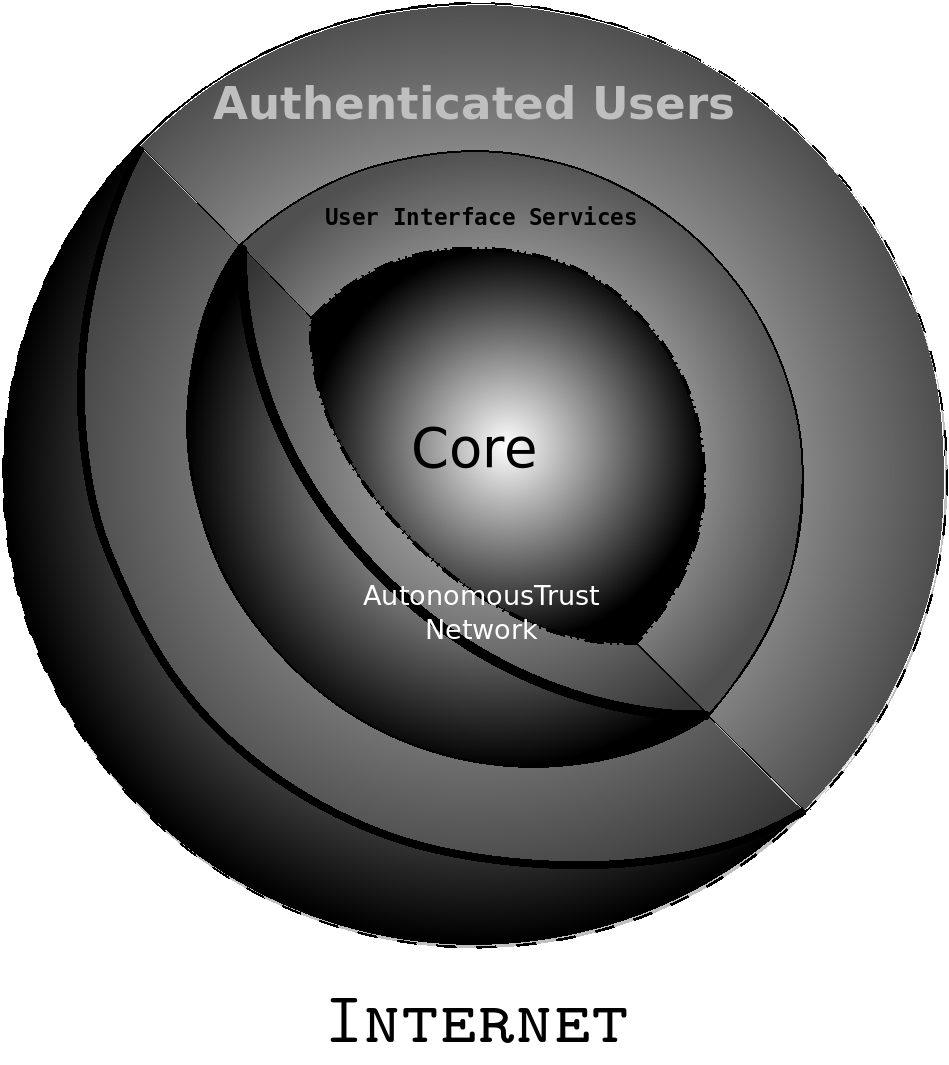
\includegraphics[width=0.4\linewidth]{users}
	\caption{User interfaces}
	\label{fig:users}
\end{figure}

Outside of the programming phase where agent capabilities are defined, user interaction with agents is strictly based on configuration (new schemas or negotiation inputs) or triggering events such as functionality or data requests, or authorizing new networks.
Users are kept in a domain separate from the main activity of the network, as seen in Figure~\ref{fig:users}.
This is a key aspect of system security, similar to CPU protection rings which restrict direct hardware access.
This clearly becomes a challenge for debugging or simply administering a system, likely solved by administrative agents.

\begin{ppl}
\input{scenario_\SCENARIO_7}
\end{ppl}